\section{Surface Integrals and the Divergence Theorem}

In \autoref{sec:line_int} we learned how to integrate along a curve. We will now learn how to perform integration over a \emph{surface} in $\mathbb{R}^{3}$, such as a sphere or a paraboloid.\index{integral!surface}\index{surface integral} Recall from \autoref{sec:vvf} how we identified points $(x,y,z)$ on a curve $C$ in $\mathbb{R}^{3}$, parametrized by $x=x(t)$, $y=y(t)$, $z=z(t)$, $a \le t \le b$, with the terminal points of the position vector
\[
 \textbf{r}(t) = x(t) \textbf{i} + y(t) \textbf{j} + z(t) \textbf{k} \text{ for $t$ in $[a,b]$.}
\]

The idea behind a parametrization of a curve is that it ``transforms'' a subset of $\mathbb{R}^{1}$ (normally an interval $[a,b]$) into a curve in $\mathbb{R}^{2}$ or $\mathbb{R}^{3}$ (see \autoref{fig:curveparam}).

\begin{lxfigure}
 \flushinner{%
  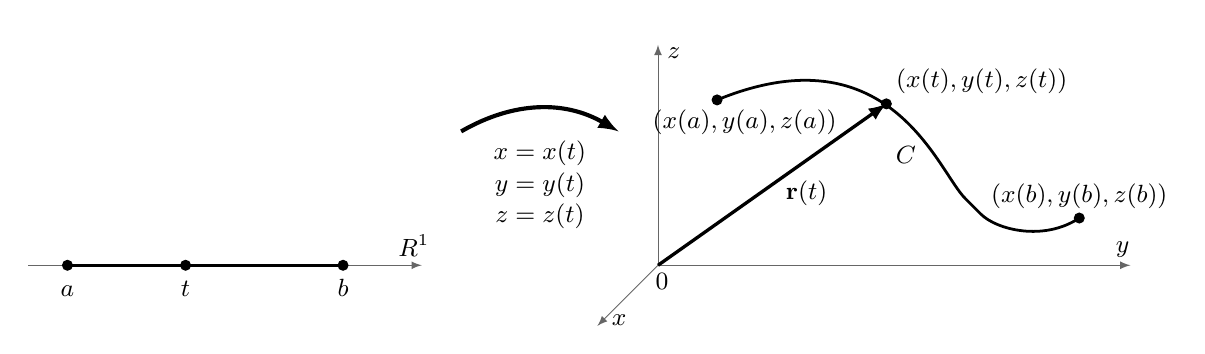
\begin{tikzpicture}
   \usetikzlibrary{arrows}
   \draw [black!60,line width=0.3pt,-latex,anchor=base] (-2,0) -- (3,0,0)
    node[black,shift={(0,-0.4)}] at (-1.5,0) {\small $a$}
    node[black,shift={(0,-0.4)}] at (0,0) {\small $t$}
    node[black,shift={(0,-0.4)}] at (2,0) {\small $b$};
   \pgfputat{\pgfpointxyz{2.9}{0.25}{0}}{\pgfbox[center,center]{\small $\mathbb{R}^{1}$}};
   \draw [line width=1.2pt] (-1.5,0) -- (2,0);
   \fill (-1.5,0) circle (2pt);
   \fill (0,0) circle (2pt);
   \fill (2,0) circle (2pt);
   \draw [black!60,line width=0.3pt,-latex] (6,0) -- (12,0,0);
   \draw [black!60,line width=0.3pt,-latex] (6,0) -- (6,2.8,0);
   \draw [black!60,line width=0.3pt,-latex] (6,0) -- (6,0,2);
   \pgfputat{\pgfpointxyz{11.9}{0.2}{0}}{\pgfbox[center,center]{\small $y$}};
   \pgfputat{\pgfpointxyz{6.2}{2.7}{0}}{\pgfbox[center,center]{\small $z$}};
   \pgfputat{\pgfpointxyz{6.2}{0}{1.8}}{\pgfbox[center,center]{\small $x$}};
   \pgfputat{\pgfpointxyz{6.05}{-0.2}{0}}{\pgfbox[center,center]{\small $0$}};
   \draw [rounded corners,line width=1pt](6.75,2.1) .. controls (8.95,3) and (9.55,1.2) .. (10,0.75) ..
    controls (10.3,0.45) and (10.9,0.3) .. (11.35,0.6);
   \draw [black,line width=1.2pt,-latex] (6,0) -- (8.9,2.05);
   \node [below] at (7.1,2.1) {\small $(x(a),y(a),z(a))$};
   \node [above right] at (8.9,2.05) {\small $(x(t),y(t),z(t))$};
   \node [above] at (11.35,0.6) {\small $(x(b),y(b),z(b))$};
   \node [below right] at (7.5,1.2) {\small $\textbf{r}(t)$};
   \node [left] at (9.4,1.4) {\small $C$};
   \fill (6.75,2.1) circle (2pt);
   \fill (8.9,2.05) circle (2pt);
   \fill (11.35,0.6) circle (2pt);
   \draw [line width=1.5pt,-latex]  (3.5,1.7) to[out=30,in=150] (5.5,1.7);
   \node [below] at (4.5,1.7) {\small $x=x(t)$};
   \node [below] at (4.5,1.3) {\small $y=y(t)$};
   \node [below] at (4.5,0.9) {\small $z=z(t)$};
  \end{tikzpicture}}
 \captionof{figure}{Parametrization of a curve $C$ in $\mathbb{R}^{3}$}
 \label{fig:curveparam}
\end{lxfigure}

Similar to how we used a parametrization of a curve to define the line integral along the curve, we will use a parametrization of a surface to define a \emph{surface integral}. We will use \emph{two} variables, $u$ and $v$, to parametrize a surface $\Sigma$ in $\mathbb{R}^{3}$: $x=x(u,v)$, $y=y(u,v)$, $z=z(u,v)$, for $(u,v)$ in some region $R$ in $\mathbb{R}^{2}$ (see \autoref{fig:surfparam}).

\begin{lxfigure}
 \begin{center}
  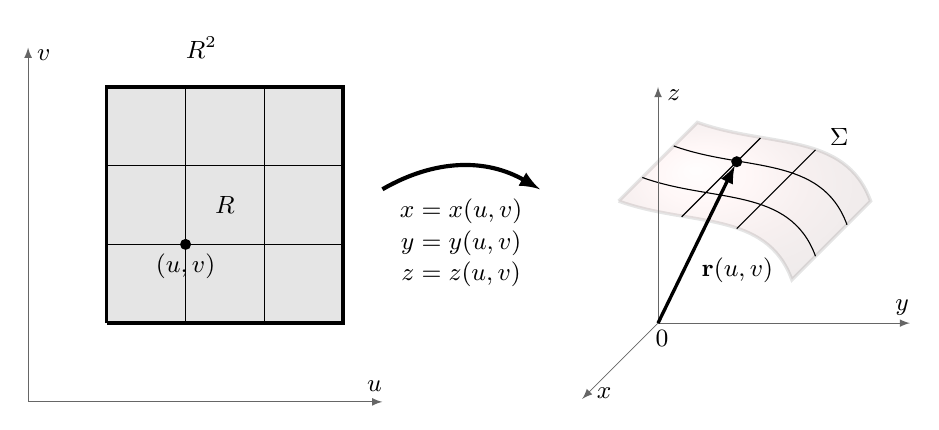
\begin{tikzpicture}
   \usetikzlibrary{arrows}
   \draw [black!60,line width=0.3pt,-latex] (0,0) -- (4.5,0);
   \draw [black!60,line width=0.3pt,-latex] (0,0) -- (0,4.5);
   \pgfputat{\pgfpointxyz{4.4}{0.2}{0}}{\pgfbox[center,center]{\small $u$}}
   \pgfputat{\pgfpointxyz{0.2}{4.4}{0}}{\pgfbox[center,center]{\small $v$}}
   \filldraw [black,line width=1.2pt,fill=black!10] (1,1) -- (1,4) -- (4,4) -- (4,1) -- (1,1);
   \draw (1,2) -- (4,2);
   \draw (1,3) -- (4,3);
   \draw (2,1) -- (2,4);
   \draw (3,1) -- (3,4);
   \node at (2.5,2.5) {\small $R$};
   \node at (2.2,4.5) {\small $\mathbb{R}^{2}$};
   \node [below] at (2,2) {\small $(u,v)$};
   \fill (2,2) circle (2pt);
   \shadedraw [line width=1.2pt,opacity=0.1,ball color=red!40] (7.5,2.55) to[out=-20,in=110] (9.7,1.55) -- (10.7,2.55)
    to[out=110,in=-20] (8.5,3.55) -- (7.5,2.55);
   \draw (7.8,2.85) to[out=-20,in=110] (10,1.85);
   \draw (8.2,3.25) to[out=-20,in=110] (10.4,2.25);
   \draw (9.3,3.35) -- (8.3,2.35);
   \draw (10,3.2) -- (9,2.2);
   \draw [black!60,line width=0.3pt,-latex] (8,1) -- (11.2,1,0);
   \draw [black!60,line width=0.3pt,-latex] (8,1) -- (8,4,0);
   \draw [black!60,line width=0.3pt,-latex] (8,1) -- (8,1,2.5);
   \pgfputat{\pgfpointxyz{11.1}{1.2}{0}}{\pgfbox[center,center]{\small $y$}};
   \pgfputat{\pgfpointxyz{8.2}{3.9}{0}}{\pgfbox[center,center]{\small $z$}};
   \pgfputat{\pgfpointxyz{8.2}{1}{2.3}}{\pgfbox[center,center]{\small $x$}};
   \pgfputat{\pgfpointxyz{8.05}{0.8}{0}}{\pgfbox[center,center]{\small $0$}};
   \node [below] at (10.3,3.6) {\small $\Sigma$};
   \fill (9,3.05) circle (2pt);
   \draw [black,line width=1.2pt,-latex] (8,1) -- (8.975,3);
   \node [below right] at (8.43,1.95) {\small $\textbf{r}(u,v)$};
   \draw [line width=1.5pt,-latex]  (4.5,2.7) to[out=30,in=150] (6.5,2.7);
   \node [below] at (5.5,2.7) {\small $x=x(u,v)$};
   \node [below] at (5.5,2.3) {\small $y=y(u,v)$};
   \node [below] at (5.5,1.9) {\small $z=z(u,v)$};
  \end{tikzpicture}
 \captionof{figure}{Parametrization of a surface $\Sigma$ in $\mathbb{R}^{3}$}
 \label{fig:surfparam}
 \end{center}
\end{lxfigure}

In this case, the position vector of a point on the surface $\Sigma$ is given by the vector-valued function
\[
 \textbf{r}(u,v) = x(u,v) \textbf{i} + y(u,v) \textbf{j} + z(u,v) \textbf{k} \text{ for $(u,v)$ in $R$.}
\]

Since $\textbf{r}(u,v)$ is a function of two variables, define the partial derivatives $\frac{\partial \textbf{r}}{\partial u}$ and $\frac{\partial \textbf{r}}{\partial v}$ for $(u,v)$ in $R$ by
\begin{align*}
 \frac{\partial \textbf{r}}{\partial u}(u,v) &=
 \frac{\partial x}{\partial u}(u,v) \textbf{i} + \frac{\partial y}{\partial u}(u,v) \textbf{j} +
 \frac{\partial z}{\partial u}(u,v) \textbf{k} ,\text{ and}\vspace{1mm}\\
 \frac{\partial \textbf{r}}{\partial v}(u,v) &=
 \frac{\partial x}{\partial v}(u,v) \textbf{i} + \frac{\partial y}{\partial v}(u,v) \textbf{j} +
 \frac{\partial z}{\partial v}(u,v) \textbf{k} .
\end{align*}

The parametrization of $\Sigma$ can be thought of as ``transforming'' a region in $\mathbb{R}^{2}$ (in the $uv$-plane) into a 2-dimensional surface in $\mathbb{R}^{3}$. This parametrization of the surface is sometimes called a \emph{patch}, based on the idea of ``patching'' the region $R$ onto $\Sigma$ in the grid-like manner shown in \autoref{fig:surfparam}.

In fact, those gridlines in $R$ lead us to how we will define a surface integral over $\Sigma$. Along the vertical gridlines in $R$, the variable $u$ is constant. So those lines get mapped to curves on $\Sigma$, and the variable $u$ is constant along the position vector $\textbf{r}(u,v)$. Thus, the tangent vector to those curves at a point $(u,v)$ is $\frac{\partial \textbf{r}}{\partial v}$. Similarly, the horizontal gridlines in $R$ get mapped to curves on $\Sigma$ whose tangent vectors are $\frac{\partial \textbf{r}}{\partial u}$.

Now take a point $(u,v)$ in $R$ as, say, the lower left corner of one of the rectangular grid sections in $R$, as shown in \autoref{fig:surfparam}. Suppose that this rectangle has a small width and height of $\Delta u$ and $\Delta v$, respectively. The corner points of that rectangle are $(u,v)$, $(u+\Delta u,v)$, $(u+\Delta u,v+\Delta v)$ and $(u,v+\Delta v)$. So the area of that rectangle is $A = \Delta u\,\Delta v$. Then that rectangle gets mapped by the parametrization onto some section of the surface $\Sigma$ which, for $\Delta u$ and $\Delta v$ small enough, will have a surface area (call it $d\sigma$) that is very close to the area of the parallelogram which has adjacent sides $\textbf{r}(u+\Delta u,v) - \textbf{r}(u,v)$ (corresponding to the line segment from $(u,v)$ to $(u+\Delta u,v)$ in $R$) and $\textbf{r}(u,v+\Delta v) - \textbf{r}(u,v)$ (corresponding to the line segment from $(u,v)$ to $(u,v+\Delta v)$ in $R$). By combining our usual notion of a partial derivative (see \autoref{def:partial_derivative} in \autoref{sec:partial_derivatives}) with that of the derivative of a vector-valued function (see \autoref{def:vvf_derivative} in \autoref{sec:vvf_calc}) applied to a function of two variables, we have
\begin{align*}
 \frac{\partial \textbf{r}}{\partial u} &\approx \frac{\textbf{r}(u+\Delta u,v) - \textbf{r}(u,v)}{\Delta u} ,\text{ and}\vspace{1mm}\\
 \frac{\partial \textbf{r}}{\partial v} &\approx \frac{\textbf{r}(u,v+\Delta v) - \textbf{r}(u,v)}{\Delta v} ,
\end{align*}
and so the surface area element $d\sigma$ is approximately
\begin{multline*}
 \norm{\Crossprod{(\textbf{r}(u+\Delta u,v) - \textbf{r}(u,v))}{(\textbf{r}(u,v+\Delta v) - \textbf{r}(u,v))}} \\
 \approx
 \norm{\Crossprod{(\Delta u \frac{\partial \textbf{r}}{\partial u})}{(\Delta v\frac{\partial \textbf{r}}{\partial v})}}
 = \norm{\Crossprod{\frac{\partial \textbf{r}}{\partial u}}{\frac{\partial \textbf{r}}{\partial v}}}\,
 \Delta u \, \Delta v
\end{multline*}
by \autoeqref{eq:crossp1}. Thus, the total surface area $S$ of $\Sigma$ is approximately the sum of all the quantities $\norm{\Crossprod{\frac{\partial \textbf{r}}{\partial u}}{\frac{\partial \textbf{r}}{\partial v}}}\,\Delta u\,\Delta v$, summed over the rectangles in $R$. Taking the limit of that sum as the diagonal of the largest rectangle goes to $0$
gives
\[
 S = \iint_{R}\,\norm{\Crossprod{\frac{\partial \textbf{r}}{\partial u}}{\frac{\partial \textbf{r}}{\partial v}}}
 \,du\,dv .
\]
We will write the double integral on the right using the special notation
\[
 \iint_{\Sigma} d\sigma =
 \iint_{R}\,\norm{\Crossprod{\frac{\partial \textbf{r}}{\partial u}}{\frac{\partial \textbf{r}}{\partial v}}}
 \,du\,dv .
\]
This is a special case of a \emph{surface integral} over the surface $\Sigma$, where the surface area element $d\sigma$ can be thought of as $1\,d\sigma$. Replacing $1$ by a general real-valued function $f(x,y,z)$ defined in $\mathbb{R}^{3}$, we have the following:

\definition{defn:surfintreal}{Scalar Surface Integral}{Let $\Sigma$ be a surface in $\mathbb{R}^{3}$ parametrized by $x=x(u,v)$, $y=y(u,v)$, $z=z(u,v)$, for $(u,v)$ in some region $R$ in $\mathbb{R}^{2}$. Let $\textbf{r}(u,v) = x(u,v) \textbf{i} + y(u,v) \textbf{j} + z(u,v) \textbf{k}$ be the position vector for any point on $\Sigma$, and let $f(x,y,z)$ be a real-valued function defined on some subset of $\mathbb{R}^{3}$ that contains $\Sigma$. The \textbf{surface integral} of $f(x,y,z)$ over $\Sigma$ is
  \[
   \iint_{\Sigma} f(x,y,z)\,d\sigma = \iint_{R} f(x(u,v),y(u,v),z(u,v))\,
   \norm{\Crossprod{\frac{\partial \textbf{r}}{\partial u}}{\frac{\partial \textbf{r}}{\partial v}}}\,du\,dv .
  \]
  In particular, the surface area $S$ of $\Sigma$ is\index{integral!surface}\index{surface integral}
  \[S = \iint_{\Sigma} 1\,d\sigma .\]}

\example{ex_surf_int}{Computing a Surface Integral}{A \emph{torus} $T$ is a surface obtained by revolving a circle of radius $a$ in the $yz$-plane around the $z$-axis, where the circle's center is at a distance $b$ from the z-axis ($0<a<b$), as in \autoref{fig:torus}. Find the surface area of $T$.\index{torus}%
% 
 \begin{lxfigure}
 \begin{center}
 \begin{tabular}{cc}
 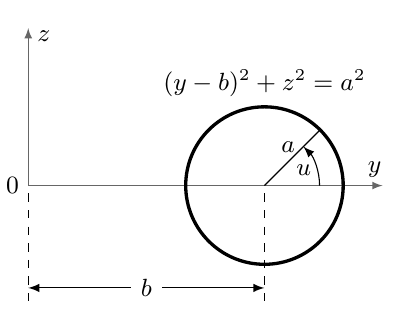
\begin{tikzpicture}
  \usetikzlibrary{arrows}
  \draw [black!60,line width=0.3pt,-latex] (0,0) -- (4.5,0);
  \draw [black!60,line width=0.3pt,-latex] (0,0) -- (0,2);
  \pgfputat{\pgfpointxyz{4.4}{0.2}{0}}{\pgfbox[center,center]{\small $y$}}
  \pgfputat{\pgfpointxyz{0.2}{1.9}{0}}{\pgfbox[center,center]{\small $z$}}
  \pgfputat{\pgfpointxyz{-0.2}{0}{0}}{\pgfbox[center,center]{\small $0$}}
  \draw [line width=1.2pt] (3,0) circle (1);
  \draw (3,0) -- (3.707,0.707);
  \draw [-latex] (3.7,0) arc (0:45:0.7);
  \node [above] at (3.3,0.3) {\small $a$};
  \node [above] at (3,1) {\small $(y-b)^2 + z^2 = a^2$};
  \node at (3.5,0.2) {\small $u$};
  \draw [dashed] (0,-0.1) -- (0,-1.5);
  \draw [dashed] (3,-0.1) -- (3,-1.5);
  \node at (1.5,-1.3) {\small $b$};
  \draw [-latex] (1.7,-1.3) -- (3,-1.3);
  \draw [-latex] (1.3,-1.3) -- (0,-1.3);
 \end{tikzpicture}
 &
 todo make a torus graphic
 %\includegraphics{torus.0}
 \\
 Circle in the $yz$-plane & Torus $T$
 \end{tabular}
 \captionof{figure}{Creating a torus}
 \label{fig:torus}
 \end{center}
\end{lxfigure}}{%
For any point on the circle, the line segment from the center of the circle to that point makes an angle $u$ with the $y$-axis in the positive $y$ direction (see \autoref{fig:torus}(a)). And as the circle revolves around the $z$-axis, the line segment from the origin to the center of that circle sweeps out an angle $v$ with the positive $x$-axis (see \autoref{fig:torus}(b)). Thus, the torus can be parametrized as:
\[
 x = (b+a\cos u)\cos v ,\quad y = (b+a\cos u)\sin v ,\quad z = a\sin u,\quad 0\le u\le 2\pi,\quad 0\le v\le 2\pi
\]
So for the position vector
\begin{align*}
 \textbf{r}(u,v) &= x(u,v) \textbf{i} + y(u,v) \textbf{j} + z(u,v) \textbf{k}\\
 &= (b+a\cos u)\cos v \,\textbf{i} + (b+a\cos u)\sin v \,\textbf{j} + a\sin u \,\textbf{k}
\end{align*}
we see that
\begin{align*}
 \frac{\partial \textbf{r}}{\partial u} &=
  -a\sin u\,\cos v \,\textbf{i} - a\sin u\,\sin v \,\textbf{j} + a\cos u \,\textbf{k}\\[6pt]
 \frac{\partial \textbf{r}}{\partial v} &=
  -(b+a\cos u)\sin v \,\textbf{i} + (b+a\cos u)\cos v \,\textbf{j} + 0 \textbf{k} ,
\end{align*}
and so computing the cross product gives
\[
 \Crossprod{\frac{\partial \textbf{r}}{\partial u}}{\frac{\partial \textbf{r}}{\partial v}} =
  -a(b+a\cos u)\cos v\,\cos u \,\textbf{i} - a(b+a\cos u)\sin v\,\cos u\,\textbf{j} - a(b+a\cos u)\sin u \,\textbf{k} ,
\]
which has magnitude
\[
 \norm{\Crossprod{\frac{\partial \textbf{r}}{\partial u}}{\frac{\partial \textbf{r}}{\partial v}}} = a(b+a\cos u) .
\]
Thus, the surface area of $T$ is
\begin{align*}
 S &= \iint_{\Sigma} 1\,d\sigma\\[6pt]
  &= \int_0^{2\pi} \int_0^{2\pi}\,\norm{\Crossprod{\frac{\partial \textbf{r}}{\partial u}}{\frac{\partial
  \textbf{r}}{\partial v}}}\,du\,dv\\[6pt]
  &= \int_0^{2\pi} \int_0^{2\pi} a(b+a\cos u)\,du\,dv\\[6pt]
  &= \int_0^{2\pi} \left( abu + a^2 \sin u \,\Big|_{u=0}^{u=2\pi}\,\right)\,dv\\[6pt]
  &= \int_0^{2\pi} 2\pi ab\,dv\\
  &= 4\pi^2 ab\eoehere
\end{align*}}

Since $\frac{\partial \textbf{r}}{\partial u}$ and $\frac{\partial \textbf{r}}{\partial v}$ are tangent to the surface $\Sigma$ (i.e. lie in the tangent plane to $\Sigma$ at each point on $\Sigma$), then their cross product $\Crossprod{\frac{\partial \textbf{r}}{\partial u}}{\frac{\partial \textbf{r}}{\partial v}}$ is perpendicular to the tangent plane to the surface at each point of $\Sigma$. Thus,
\[
 \iint_{\Sigma} f(x,y,z)\,d\sigma = \iint_{R} f(x(u,v),y(u,v),z(u,v))\,\norm{\textbf{n}}\,d\sigma ,
\]
where $\textbf{n} = \Crossprod{\frac{\partial \textbf{r}}{\partial u}}{\frac{\partial \textbf{r}}{\partial v}}$. We say that \textbf{n} is a \textbf{normal vector} to $\Sigma$.\index{vector!normal}

\mtable{Outward Unit Normal Vectors}{fig_outward}{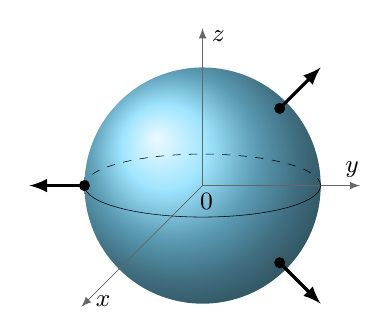
\begin{tikzpicture}
 \usetikzlibrary{arrows}
 \definecolor{spherecolor}{HTML}{80DCFF}
 \shade [ball color=spherecolor] (0,0) circle (1.5);
 \draw [black!60,line width=0.3pt,-latex] (0,0) -- (2,0,0);
 \draw [black!60,line width=0.3pt,-latex] (0,0) -- (0,2,0);
 \draw [black!60,line width=0.3pt,-latex] (0,0) -- (0,0,4);
 \pgfputat{\pgfpointxyz{1.9}{0.2}{0}}{\pgfbox[center,center]{\small $y$}};
 \pgfputat{\pgfpointxyz{0.2}{1.9}{0}}{\pgfbox[center,center]{\small $z$}};
 \pgfputat{\pgfpointxyz{0.2}{0}{3.8}}{\pgfbox[center,center]{\small $x$}};
 \pgfputat{\pgfpointxyz{0.05}{-0.2}{0}}{\pgfbox[center,center]{\small $0$}};
 \draw [line width=0.2pt] (-1.5,0) arc (180:360:1.5 and 0.4);
 \draw [dashed,line width=0.2pt] (1.5,0) arc (0:180:1.5 and 0.4);
 \fill (0.98,0.98) circle (2pt);
 \draw [line width=1.2pt,-latex] (0.98,0.98) -- (1.5,1.5);
 \fill (0.98,-0.98) circle (2pt);
 \draw [line width=1.2pt,-latex] (0.98,-0.98) -- (1.5,-1.5);
 \fill (-1.5,0) circle (2pt);
 \draw [line width=1.2pt,-latex] (-1.5,0) -- (-2.2,0);
\end{tikzpicture}}
Recall that normal vectors to a plane can point in two opposite directions. By an \textbf{outward unit normal vector} to a surface $\Sigma$, we will mean the unit vector that is normal to $\Sigma$ and points away from the ``top'' (or ``outer'' part) of the surface. This is a hazy definition, but the picture in \autoref{fig_outward} gives a better idea of what outward normal vectors look like, in the case of a sphere. With this idea in mind, we make the following definition of a surface integral of a 3-dimensional \emph{vector field} over a surface:\index{outward normal}

\definition{defn:surfintvec}{Vector Surface Integral}{Let $\Sigma$ be a surface in $\mathbb{R}^{3}$ and let $\textbf{f}(x,y,z) = f_1(x,y,z) \textbf{i} + f_2(x,y,z) \textbf{j} + f_3(x,y,z) \textbf{k}$ be a vector field defined on some subset of $\mathbb{R}^{3}$ that contains $\Sigma$. The \textbf{surface integral} of \textbf{f} over $\Sigma$ is
  \begin{equation}\label{eqn:surfintvec}
   \iint_{\Sigma} \Dotprod{\textbf{f}}{d\sigma} =
   \iint_{\Sigma} \Dotprod{\textbf{f}}{\textbf{n}}\,d\sigma ,
  \end{equation}
  where, at any point on $\Sigma$, \textbf{n} is the outward unit normal vector to $\Sigma$.}

Note in the above definition that the dot product inside the integral on the right is a real-valued function, and hence we can use \autoref{defn:surfintreal} to evaluate the integral.

\example{exmp_surfintex}{Evaluating a Surface Integral}{Evaluate the surface integral $\iint_{\Sigma} \Dotprod{\textbf{f}}{d\sigma}$, where $\textbf{f}(x,y,z) = yz\textbf{i} + xz\textbf{j} + xy\textbf{k}$ and $\Sigma$ is the part of the plane $x+y+z=1$ with $x \ge 0$, $y \ge 0$, and $z \ge 0$, with the outward unit normal $\textbf{n}$ pointing in the positive $z$ direction (see \autoref{fig_surf_plane}).%
 \mtable{The surface in \autoref{exmp_surfintex}}{fig_surf_plane}{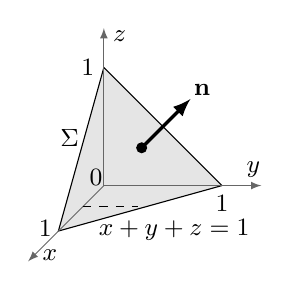
\begin{tikzpicture}
  \usetikzlibrary{arrows}
  \filldraw [black,fill=black!10] (1.5,0,0) -- (0,1.5,0) -- (0,0,1.5) -- (1.5,0,0);
  \draw [black!60,line width=0.3pt,-latex] (0,0) -- (2,0,0);
  \draw [black!60,line width=0.3pt,-latex] (0,0) -- (0,2,0);
  \draw [black!60,line width=0.3pt,-latex] (0,0) -- (0,0,2.5);
  \pgfputat{\pgfpointxyz{1.9}{0.2}{0}}{\pgfbox[center,center]{\small $y$}};
  \pgfputat{\pgfpointxyz{0.2}{1.9}{0}}{\pgfbox[center,center]{\small $z$}};
  \pgfputat{\pgfpointxyz{0.2}{0}{2.3}}{\pgfbox[center,center]{\small $x$}};
  \pgfputat{\pgfpointxyz{-0.1}{0.1}{0}}{\pgfbox[center,center]{\small $0$}};
  \node [below] at (1.5,0,0) {\small $1$};
  \node [left] at (0,1.5,0) {\small $1$};
  \node [left] at (0,0,1.4) {\small $1$};
  \node [left] at (0,0.8,0.5) {\small $\Sigma$};
  \node [below] at (1.2,0,0.8) {\small $x+y+z=1$};
  \draw [dashed] (0,0,0.7) -- (0.7,0,0.7);
  \fill (0.48,0.48) circle (2pt);
  \draw [line width=1.2pt,-latex] (0.48,0.48) -- (1.1,1.1);
  \node [above right] at (1.02,1.02) {\small $\textbf{n}$};
 \end{tikzpicture}}}{%
 Since the vector $\textbf{v} = (1,1,1)$ is normal to the plane $x+y+z=1$ (why?), then dividing \textbf{v} by its length yields the outward unit normal vector $\textbf{n} = \left( \frac{1}{\sqrt{3}}, \frac{1}{\sqrt{3}},\frac{1}{\sqrt{3}} \right)$. We now need to parametrize $\Sigma$. As we can see from Figure 4.4.5, projecting $\Sigma$ onto the $xy$-plane yields a triangular region $R= \lbrace\,(x,y): 0 \le x \le 1, 0 \le y \le 1-x\,\rbrace$. Thus, using $(u,v)$ instead of $(x,y)$, we see that
 \[x=u, y=v, z=1-(u+v),\text{ for } 0 \le u \le 1, 0 \le v \le 1-u\]
 is a parametrization of $\Sigma$ over $R$ (since $z=1-(x+y)$ on $\Sigma$). So on $\Sigma$,
 \begin{align*}
  \Dotprod{\textbf{f}}{\textbf{n}} &=
   \Dotprod{(yz,xz,xy)}{\left( \frac{1}{\sqrt{3}},\frac{1}{\sqrt{3}},\frac{1}{\sqrt{3}} \right)}
   = \frac{1}{\sqrt{3}}(yz+xz+xy)\\[8pt]
   &= \frac{1}{\sqrt{3}}((x+y)z+xy)
   = \frac{1}{\sqrt{3}}((u+v)(1-(u+v))+uv)\\[8pt]
   &= \frac{1}{\sqrt{3}}((u+v)- (u+v)^2 + uv)
 \end{align*}
 for $(u,v)$ in $R$, and for $\textbf{r}(u,v)=x(u,v)\textbf{i} + y(u,v)\textbf{j} + z(u,v)\textbf{k} = u\textbf{i} + v\textbf{j} + (1-(u+v))\textbf{k}$ we have
 \[
  \Crossprod{\frac{\partial \textbf{r}}{\partial u}}{\frac{\partial \textbf{r}}{\partial v}} =
   \Crossprod{(1,0,-1)}{(0,1,-1)} = (1,1,1) \quad\Rightarrow\quad
   \norm{\Crossprod{\frac{\partial \textbf{r}}{\partial u}}{\frac{\partial \textbf{r}}{\partial v}}} = \sqrt{3}.
 \]
 Thus, integrating over $R$ using vertical slices (e.g. as indicated by the dashed line in \autoref{fig_surf_plane}) gives
 \begin{align*}
  \iint_{\Sigma} \Dotprod{\textbf{f}}{d\sigma} &=
   \iint_{\Sigma} \Dotprod{\textbf{f}}{\textbf{n}}\,d\sigma\\[6pt]
   &= \iint_{R} (\Dotprod{\textbf{f}(x(u,v),y(u,v),z(u,v))}{\textbf{n}})\,
    \norm{\Crossprod{\frac{\partial \textbf{r}}{\partial u}}{\frac{\partial \textbf{r}}{\partial v}}}\,dv\,du\\[6pt]
   &= \int_0^1 \int_0^{1-u} \frac{1}{\sqrt{3}}((u+v)- (u+v)^2 + uv) \sqrt{3}\,dv\,du\\[8pt]
   &= \int_0^1 \left( \left.\frac{(u+v)^2}{2} - \frac{(u+v)^3}{3} + \frac{uv^2}{2}\,\right|_{v=0}^{v=1-u} \right)\,du\\[8pt]
   &= \int_0^1 \left( \frac{1}{6} + \frac{u}{2} - \frac{3u^2}{2} + \frac{5u^3}{6} \right)\,du\\[8pt]
   &= \left.\frac{u}{6} + \frac{u^2}{4} - \frac{u^3}{2} + \frac{5u^4}{24}\,\right|_0^1 = \frac{1}{8}.\eoehere
 \end{align*}}

Computing surface integrals can often be tedious, especially when the formula for the outward unit normal vector at each point of $\Sigma$ changes. The following theorem provides an easier way in the case when $\Sigma$ is a \textbf{closed surface}, that is, when $\Sigma$ encloses a bounded solid in $\mathbb{R}^{3}$. For example, spheres, cubes, and ellipsoids are closed surfaces, but planes and paraboloids are not.\index{closed surface}

\theorem{thm:divergence}{Divergence Theorem}{\index{Divergence Theorem}%
Let $\Sigma$ be a closed surface in $\mathbb{R}^{3}$ which bounds a solid $S$, and let $\textbf{f}(x,y,z) = f_1(x,y,z) \textbf{i} + f_2(x,y,z) \textbf{j} + f_3(x,y,z) \textbf{k}$ be a vector field defined on some subset of $\mathbb{R}^{3}$ that contains $\Sigma$. Then
  \begin{equation}\label{eqn:divergence}
   \iint_{\Sigma} \Dotprod{\textbf{f}}{d\sigma} = \iiint_{S} \text{div}\textbf{f} dV ,
  \end{equation}
  where
  \begin{equation}\label{eqn:div}
   \text{div}\textbf{f} = \frac{\partial f_1}{\partial x} + \frac{\partial f_2}{\partial y} +
   \frac{\partial f_3}{\partial z}\index{divergence}
  \end{equation}
  is called the \textbf{divergence} of \textbf{f}.}

The proof of the Divergence Theorem is very similar to the proof of Green's Theorem, i.e. it is first proved for the simple case when the solid $S$ is bounded above by one surface, bounded below by another surface, and bounded laterally by one or more surfaces. The proof can then be extended to more general solids.%\footnote{See \cite[\S\,15.6]{tm} for the details.}

\example{ex_div_thm}{Using the Divergence Theorem}{Evaluate $\iint_{\Sigma} \Dotprod{\textbf{f}}{d\sigma}$, where $\textbf{f}(x,y,z) = x\textbf{i} +  y\textbf{j} + z\textbf{k}$ and $\Sigma$ is the unit sphere $x^2 + y^2 + z^2 = 1$.}{We see that $\text{div}\textbf{f} = 1+1+1=3$, so
 \begin{align*}
  \iint_{\Sigma} \Dotprod{\textbf{f}}{d\sigma} &=
  \iiint_{S} \text{div}\textbf{f} dV
  = \iiint_{S} 3 dV\\
  &= 3 \iiint_{S} 1 dV
  = 3\,\text{vol}(S) = 3\cdot \frac{4\pi (1)^3}{3} = 4\pi .\eoehere
 \end{align*}}

In physical applications, the surface integral $\iint_{\Sigma} \Dotprod{\textbf{f}}{d\sigma}$ is often referred to as the \textbf{flux} of \textbf{f} through the surface $\Sigma$. For example, if \textbf{f} represents the velocity field of a fluid, then the flux is the net quantity of fluid to flow through the surface $\Sigma$ per unit time.\index{flux} A positive flux means there is a net flow \emph{out} of the surface (i.e. in the direction of the outward unit normal vector \textbf{n}), while a negative flux indicates a net flow inward (in the direction of $-\textbf{n}$).

The term divergence comes from interpreting div \textbf{f} as a measure of how much a vector field ``diverges'' from a point. This is best seen by using another definition of div \textbf{f} which is equivalent
%\footnote{See \cite{sch}, p. 36-39, for an intuitive discussion of this.}
to the definition given by \autoeqref{eqn:div}. Namely, for a point $(x,y,z)$ in $\mathbb{R}^{3}$,
\begin{equation}\label{eqn:divalt}
 \text{div }\textbf{f}(x,y,z) = \lim_{V \to 0} \frac{1}{V} \iint_{\Sigma} \Dotprod{\textbf{f}}{d\sigma} ,
\end{equation}
where $V$ is the volume enclosed by a closed surface $\Sigma$ around the point $(x,y,z)$. In the limit, $V \to 0$ means that we take smaller and smaller closed surfaces around $(x,y,z)$, which means that the volumes they enclose are going to zero. It can be shown that this limit is independent of the shapes of those surfaces. Notice that the limit being taken is of the ratio of the flux through a surface to the volume enclosed by that surface, which gives a rough measure of the flow ``leaving'' a point, as we mentioned. Vector fields which have zero divergence are often called \emph{solenoidal}\index{solenoidal} fields.

The following theorem is a simple consequence of \autoeqref{eqn:divalt}.

\theorem{thm:divzero}{Zero Flux}{If the flux of a vector field \textbf{f} is zero through every closed surface containing a given point, then $\text{div }\textbf{f} = 0$ at that point.}

\begin{proof}
 By \autoeqref{eqn:divalt}, at the given point $(x,y,z)$ we have 
 \begin{align*}
  \text{div }\textbf{f}(x,y,z) &= \lim_{V \to 0} \frac{1}{V} \iint_{\Sigma} \Dotprod{\textbf{f}}{d\sigma}
   \text{ for closed surfaces $\Sigma$ containing $(x,y,z)$, so}\\
    &= \lim_{V \to 0} \frac{1}{V} \,\, (0) \text{ by our assumption that the flux through each $\Sigma$ is
    zero, so}\\[6pt]
    &= \lim_{V \to 0} \, 0\\
    &= 0 .\qedhere
 \end{align*}
\end{proof}

Lastly, we note that sometimes the notation
\[
 \oiint_{\Sigma} f(x,y,z)\,d\sigma \quad\text{and}\quad \oiint_{\Sigma} \Dotprod{\textbf{f}}{d\sigma}
\]
is used to denote surface integrals of scalar and vector fields, respectively, over closed surfaces.\index{$\oiint_{\Sigma}$} Especially in physics texts, it is common to see simply $\oint_{\Sigma}$ instead of $\oiint_{\Sigma}$.

\printexercises{exercises/14_Div_Thm_exercises}
